%%%%%%%%%%%%%%%%%%%%%%%%%%%%%%%%%%%%%%%%%%%%%%%%%%%%%%%%%%
\section{Motivation}
\label{sec:motivation}
%%%%%%%%%%%%%%%%%%%%%%%%%%%%%%%%%%%%%%%%%%%%%%%%%%%%%%%%%%
\begin{figure}
   {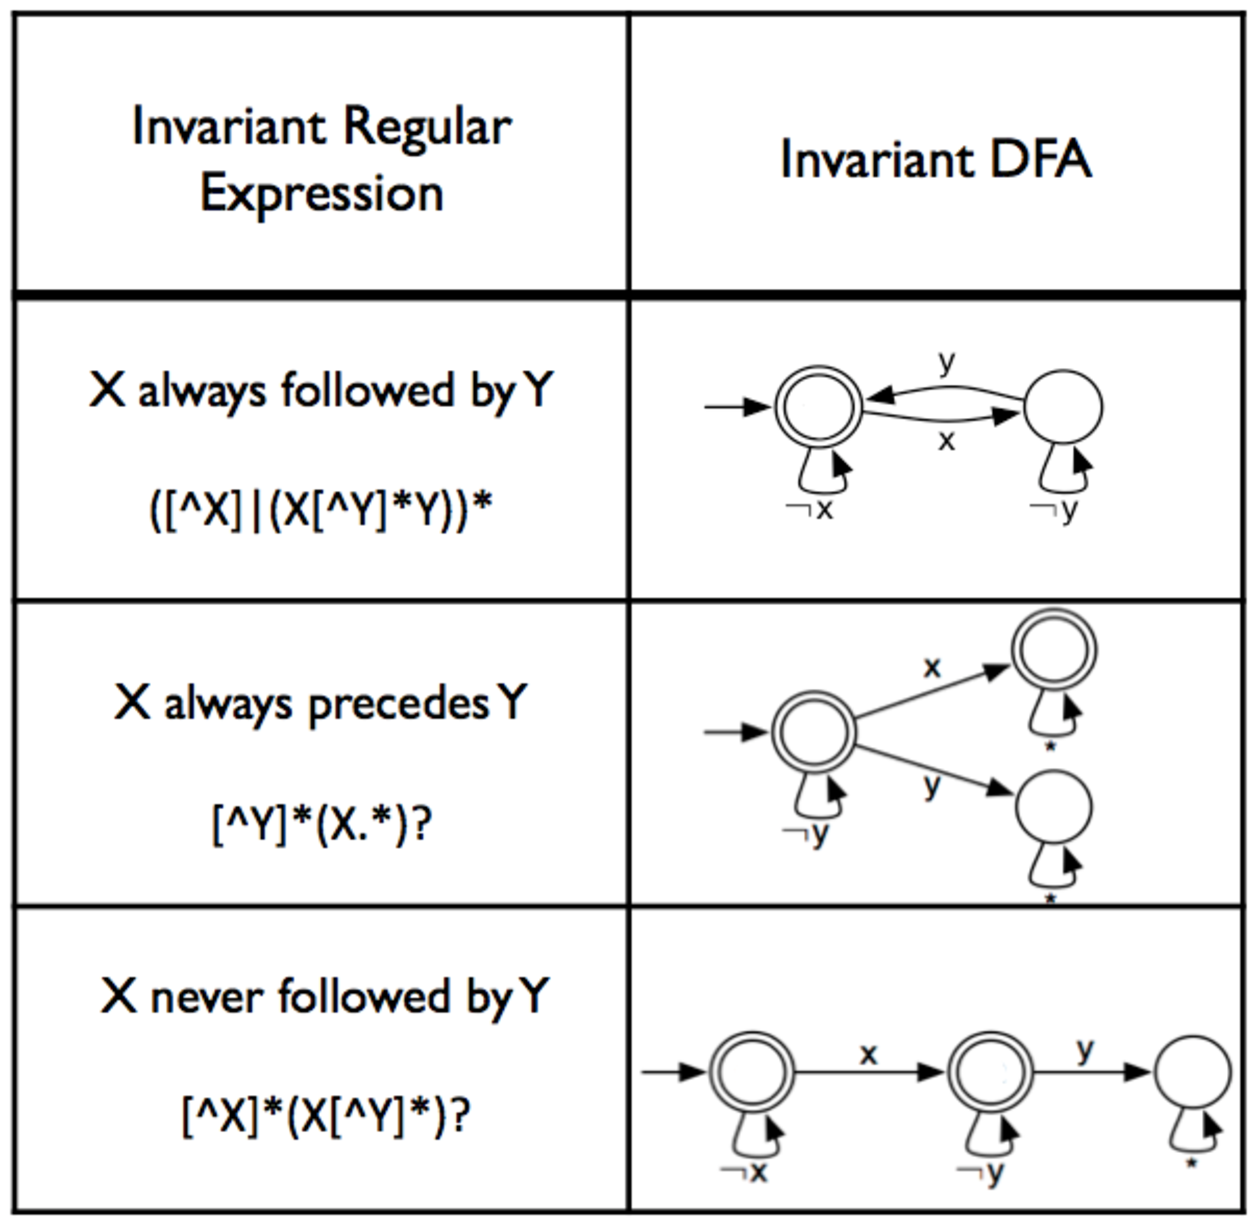
\includegraphics[width=\columnwidth]{fig/invRegexDfa.pdf}}
   \caption{The regular expressions used to translate each invariant type into
   an
   invariant DFA.
    } 
   \label{fig:invRegDfa}
\end{figure}
In addition to efficiency, the formal languages perspective is poised to improve
upon a number of other Synoptic shortcomings. 

First, Synoptic itself is not very flexible.
Built into many places of its implementation are assumptions about the three explicitly
mined invariants described in Section~\ref{sec:synoptic}. Adding a new invariant would require new invariant
miner, model checker, and counter-example generator code. So while it is
certainly possible to incorporate new invariants, there are a large
number of potentially useful invariants and each individually would require 
substantial effort to implement. 

Second, though intended for developers, Synoptic is challenging for users to
understand as the aggregate process is complex. For the final model to be most
helpful, we believe that users would benefit from understanding the process
that generated the model.

Finally, there is not a known optimal way to choose the order in which
invariants are satisfied during Synoptic's refinement phase. This problem
introduces nondeterminism into the process, as the order in which invariants are
satisfied affects the final model and can cause non-optimal refinement
steps. Synoptic is thus not guaranteed to find a globally minimal 
model satisfying all invariants, and will generate an arbitrary locally minimal
model. Because smaller models are easier to analyze,
the global minimum is preferred. 

As we will soon see, InvariMint addresses each of these deficiencies. But first, a
more formal treatment of its approach.
